\chapter{Out-of-core Octree}
\label{chap:octree}


\section{Overview}

Modern point clouds are often too large to fit into memory, let alone video memory. In order to manage datasets whose size exceeds the available system memory, the data must be stored in a structured file, such that data can be loaded into memory in chunks efficiently. A structure that partitions data into usable chunks that share spatial properties is an octree. 
An octree is a hierarchical datastructure in which each node represents a spatial region, defined by a three-dimensional bounding box. If the decision is made to split a node, eight children are created, each representing an octant of the parent's bounding box.


\section{Node Split Ruling}

Numerous decision rules exist that determine whether a node should be split. A node is split if the point count exceeds a threshold $n$.  For various reason, a decision based on the number of points in a node is favored. In order to keep the amount of streamed data roughly the same and have loading times vary only a little, chunks of data should be of roughly the same size as well. This allows to estimate the load time in advantage since the approximate size of a chunk is known. Having nodes of mostly the same size allows the runtime of procedures that heavily depend on the size of the node to be consistent . In this application, a point count $n = 5000$ is chosen. 
\\
\\
If a node is partitioned, it's elements are replaced by a random subset of points of size $n$ from its children, thus creating an efficient \textit{level-of-detail} representation of the point cloud on multiple scales. 
Other implementations, such as Potree\cite{SCHUETZ-2016-POT}, where some points remain in the parent instead of being stored in a child node, are more efficient in terms of disc space. However, in this application, each node can be viewed as self-contained, such that no points from predecessor nodes are needed to fully represent the point cloud for this region and \textit{level-of-detail}. 


\section{Out-of-core Functionalities}

\textit{Out-of-core} describes a way of handling datasets that are too large to fit into system memory. Small chunks of data are loaded into memory on demand, while the largest part of the dataset remains on the hard drive. If an octree node is loaded into memory, its content remains on the disc until needed. This allows to quickly interact with nodes without loading data. Even child nodes are stored on the hard drive and are loaded into memory on demand. 
Loading data into memory can only be done as long as free memory is available. Unused memory is freed periodically after it was not accessed for a certain amount of time. 


\section{Octree Postprocessing}

Common point cloud datasets mostly only contain information on position and color and lack distinct geometric features such as normal vectors. Normal vectors are significant for shape detection, since they introduce information on the local curvature to the point cloud.  In order to enrich the dataset with additional information, some calculations are performed after the octree build process is complete. 


\subsection{rkd-Tree}

A rkd-tree by Tobler\cite{tobler2011rkd} is an efficient datastructure for point queries. While the octree partitions the space into fairly small regions, the rkd-tree is used to easily find points within a node at a certain location. 


\subsection{Normals}

For lighting and shape detection, each point must possess a normal vector. A point's normal is determined by the local neighborhood. Using the node's rkd-tree a $k$-nearest-neighbor search is performed to get the $k$ closest neighbors. Principal Component Analysis\cite{jolliffe2002principal} is used to fit a plane into the neighborhood. The plane's normal is used as the point's normal.


\subsection{Centroid}

The centroid of a node provides an indicator on the distribution of points in the octree node. The centroid can be used as a target for the camera to focus on the presumably most dense part of the point cloud. 


\subsection{Density}

The density describes the average distance between a point and its nearest neighbor. The density increases with higher \textit{level-of-detail} since more points are contained in a smaller region. To find the nearest neighbor, again, the node's rkd-tree is used. 


\section{Octree Culling and Render Horizon}
\label{sec:renderHorizon}

As a point cloud normally contains more data than the GPU is able to render, only nodes are rendered that contribute to the currently viewed scene. The result of this operation is a new octree that contains only nodes that are currently rendered. 
\\
\\
A simple, yet powerful culling heuristic is view frustum culling. Nodes that are outside of the view frustum are not rendered. By using view frustum culling, complete branches of the octree are removed, however, the remaining branches are still too large to be rendered completely. A \textit{level-of-detail} decision function determines if a node should be rendered. Depending on the node's distance to the nearplane and its volume a decision is made if the node should be rendered or not. 

\begin{figure}
    \centering
    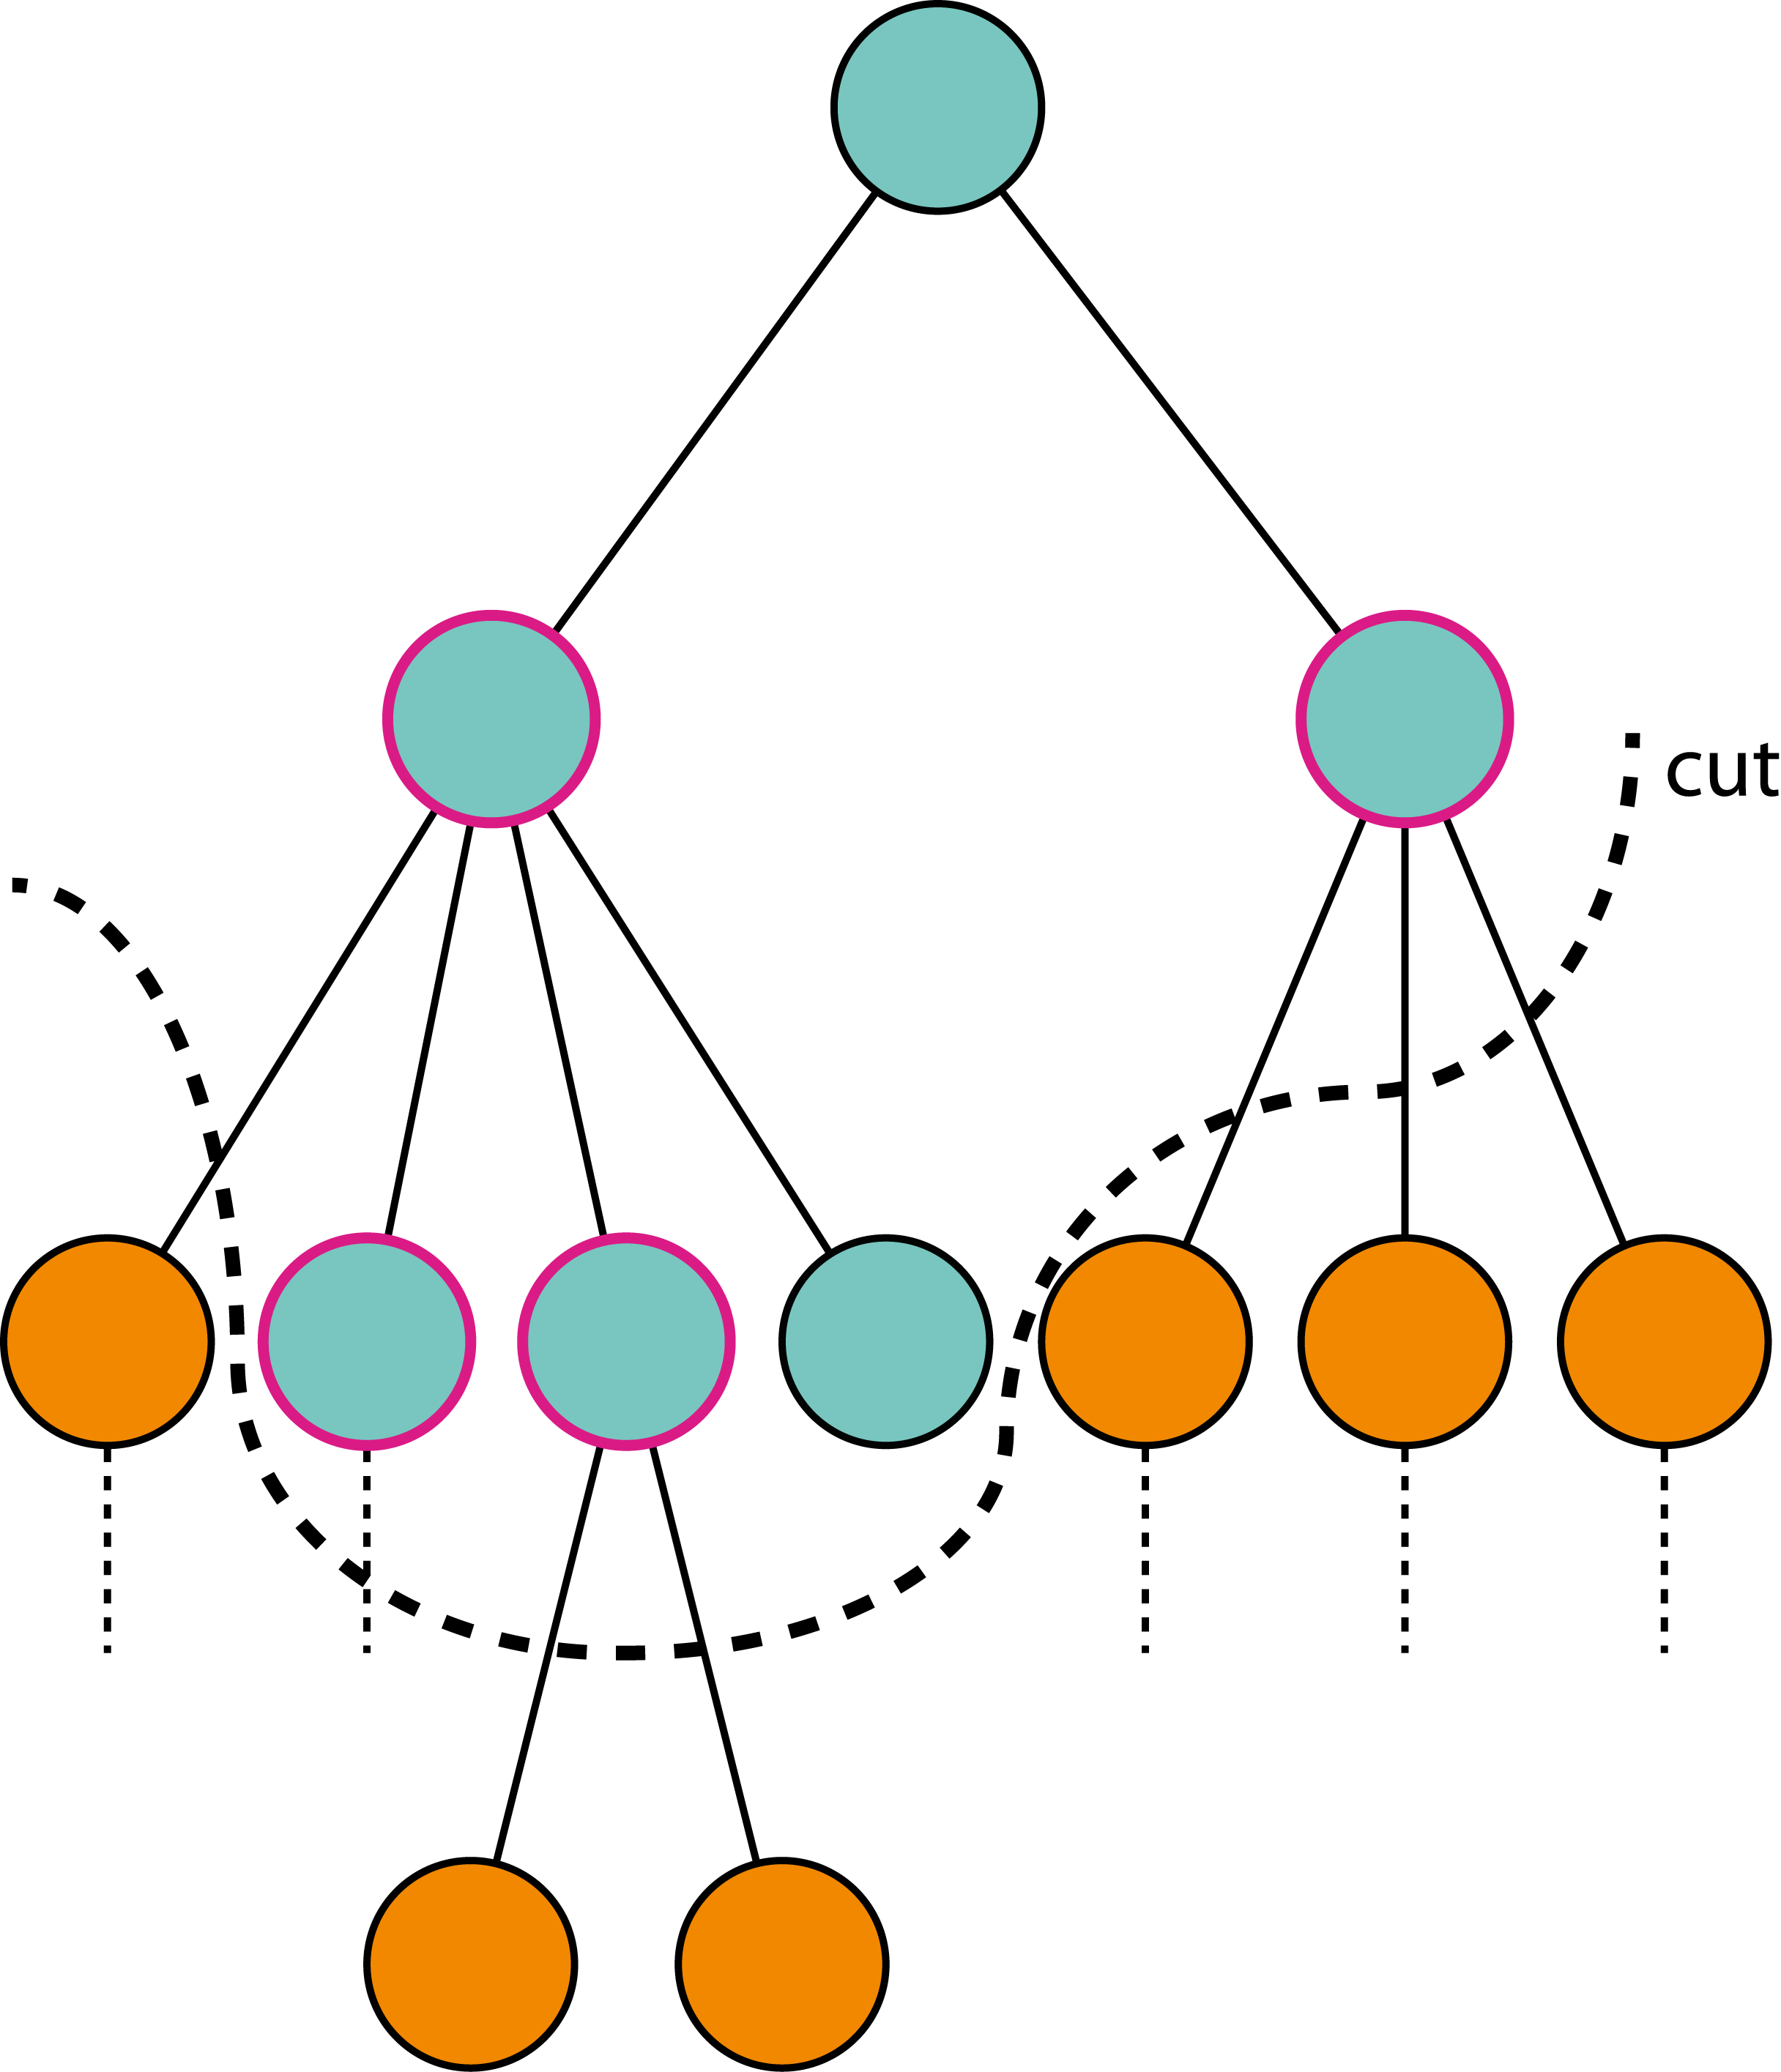
\includegraphics[width=0.5\textwidth]{Octree/renderHorizon.png}
    \caption{The render horizon of an octree is showcased as a dashed line. Nodes that are rendered, are colored in turquoise, nodes that are part of the render horizon, are bordered in magenta. }
    \label{fig:renderHorizon}
\end{figure}


The \textit{Render horizon} describes a cut that separates the octree into a rendered part and an unrendered part. The nodes of which some of the children are affected by the cut create the render horizon. Nodes along the render horizon share the property that one of its direct children contains points that are are not rendered anymore. This property is useful when additional information should be displayed. 
\\
Figure \ref{fig:renderHorizon} showcases an exemplary cut, displayed as a dashed line, through an octree along with its created render horizon. Nodes that are rendered, are colored in turquoise. A dashed line originating from a node indicates that the node contains children which are not rendered. Nodes whose border is colored in magenta belong to the set of nodes of the render horizon. Those nodes contain edges that are intersected by the cut. 
\\
As the rendered parts of the octree are needed for multiple tasks in the application, culling is performed only once per frame. The result of the culling procedure is an octree that only contains the nodes that are currently rendered, thus interactions that rely on visible data must only be performed on this octree without performing culling operations twice. 